\newpage
\hypertarget{rules vis}{}
\subsection{Visual Rules}
\visHeader

It should be noted that each rule needs to define the actions of its \texttt{source}, \texttt{target}, and \texttt{correspondence} metamodels. These are
differentiated in EA spatially.

\subsection{BoxToDictionaryRule}

\begin{enumerate}

\item[$\blacktriangleright$] In EA, open the \texttt{Rules} diagram of your TGG project, automatically generated when you first created the integration package.
Create your first rule by either holding \texttt{ctrl} while you click in the diagram, or drag-and-drop the \texttt{Rule} item from the TGG toolbox to the left
of the diagram window (Fig.~\ref{fig:create_tgg_rule}). Press \texttt{alt + enter} to raise its \texttt{Properties} dialogue, and update its name to
\texttt{BoxToDictionaryRule}.

\vspace{0.5cm}

\begin{figure}[htbp]
\begin{center}
  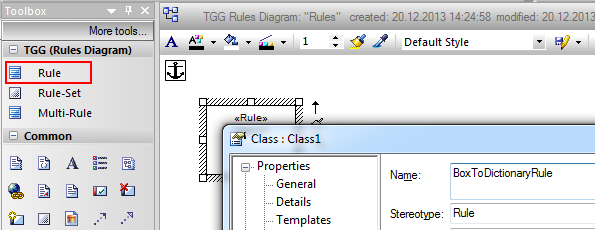
\includegraphics[width=\textwidth]{ea_TGGNewRule}
  \caption{Creating a TGG rule}
  \label{fig:create_tgg_rule}
\end{center}
\end{figure}

\item[$\blacktriangleright$] Double click the element to open the \texttt{BoxToDictionaryRule} diagram. Drag-and-drop the \texttt{Box} EClass from the project
browser into the diagram, choosing to paste the element as an \texttt{instance}.\footnote{If the 'Paste Element' dialogue doesn't appear, hold \texttt{ctrl} and
confirm you haven't selected the autosave option under \texttt{options}.} The \texttt{name} and \texttt{binding operator} should already be set to \texttt{box}
and \texttt{create}.

\item[$\blacktriangleright$] Repeat the action to create an instance of \texttt{Dictionary}.

\item[$\blacktriangleright$] Quick-link from \texttt{box} to \texttt{dictionary} and create a TGG Correspondence link. To keep things simple, keep the name 
\texttt{boxToDictionary} and select the \texttt{BoxToDictionary} correspondence type from the drop-down list which you declared in the schema.

\newpage

Believe it or not, our rule \emph{already} creates a \texttt{Box}, \texttt{Dictionary}, and correspondence link between them at the same time, as-is!
Unfortunately, this only creates the objects, and doesn't relate any of their attributes. Why don't we try to connect the \texttt{name} of the \texttt{box} to
the \texttt{title} of the dictionary so that they always match? 

For this, we can once again use \emph{attribute constraints}!\footnote{First defined in Part III, Section 4} When used with TGG rules, attribute constraints
provide a bidirectional and high-level solution for attribute manipulation. We're looking for a constraint which ensures that \texttt{box.name} and
\texttt{dictionary.title} are consistent.

\vspace{0.5cm}

\item[$\blacktriangleright$] Following the process of creating a new \texttt{Rule}, either hold \texttt{ctrl} and click in the diagram to raise a context menu
of the current toolbox and select \texttt{TGG Constraint} (Fig.~\ref{fig:common_toolbox}), or drag-and-drop a \emph{TGG Constraint} from the actual toolbox to
the left of the window.

\vspace{0.5cm}

\begin{figure}[htbp]
\begin{center}
  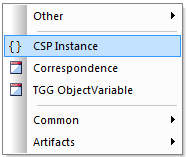
\includegraphics[width=0.3\textwidth]{ea_createTGGConstraint}
  \caption{Constraint from the Toolbox in EA}
  \label{fig:common_toolbox}
\end{center}
\end{figure}

\item[$\blacktriangleright$] Double click the empty box to open its \texttt{TGGConstraint Dialog}. There's a pre-populated list of available constraints; Choose
\texttt{eq} (equals) and double-click each of the \texttt{Value} fields to specify the \texttt{a} and \texttt{b} values as depicted in
Fig.~\ref{fig:first_tgg_constraint}. Press \texttt{Add} to save the constraint, affirming with \texttt{OK}.

\item[$\blacktriangleright$] Your rule should now resemble Fig.~\ref{fig:tgg_rule_with_constraint}, where the new links represent the object dependencies in the
constraint.

\newpage

\begin{figure}[htbp]
\begin{center}
  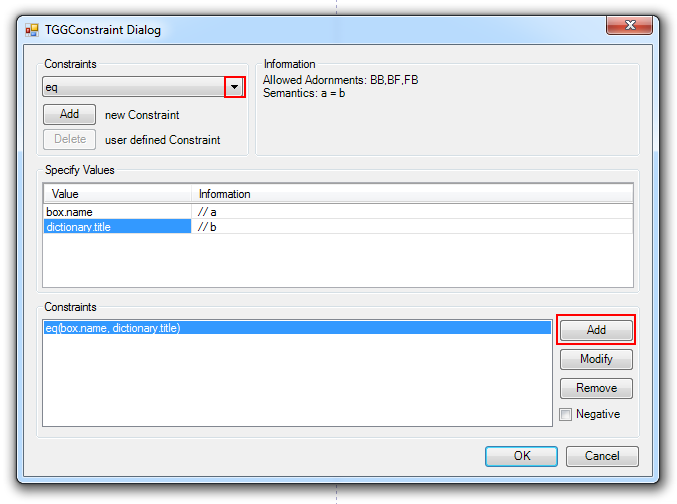
\includegraphics[width=\textwidth]{ea_TGGConstraintDialog}
  \caption{Creating a Constraint in EA}
  \label{fig:first_tgg_constraint}
\end{center}
\end{figure}

\vspace{1cm}

\begin{figure}[h!]
\begin{center}
  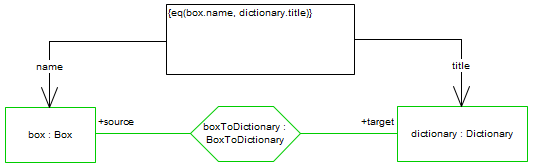
\includegraphics[width=\textwidth]{ea_TGGconstraintDependency}
  \caption{A TGG Rule with a Constraint}
  \label{fig:tgg_rule_with_constraint}
  \end{center}
\end{figure}

\newpage

Our first TGG Rule is not yet complete! Remember, we still need to create the initial structure of the learning box. In contrast to the rather
simple dictionary, where \texttt{Dictionary} is a direct container for ever \texttt{Entry} object, we have to create a number of connected \texttt{Partitions}
that hold the \texttt{Cards} in the learning box. 

\item[$\blacktriangleright$] Given that there are are three valid difficulty levels for every \texttt{Entry}, create three \texttt{Partition} object variables,
complete with appropriate link variables that satisfy the Leitner's Box rules (the \texttt{next}, \texttt{previous}, and \texttt{box} references). Your TGG rule
should come to resemble Fig.~\ref{fig:boxtodictionaryrule_complete}.


\begin{figure}[htbp]
\begin{center}
  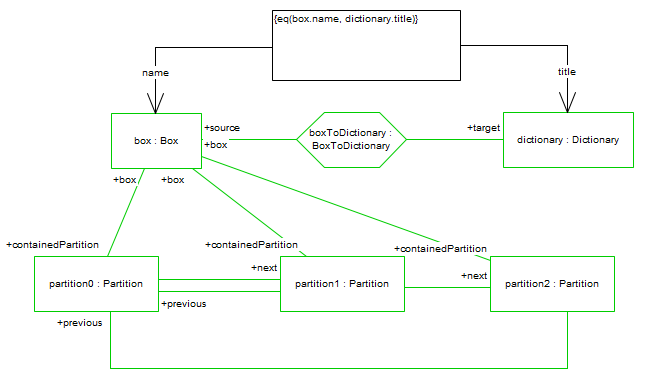
\includegraphics[width=1.1\textwidth]{ea_TGGCompleteRule}
  \caption{Complete TGG rule diagram for \texttt{BoxToDictionaryRule}}
  \label{fig:boxtodictionaryrule_complete}
\end{center}
\end{figure}

\end{enumerate}


Fantastic work! The first concept of our transformation is complete! If you are in hurry, you can jump ahead and proceed to Section~\ref{sect:TGGs_in_Action}:
TGGs in Action. There you can transform a box to a dictionary and vice-versa, but please be aware that your specified TGG (with just one rule) will only be
able to cope with empty boxes and dictionaries. Handling additional elements (i.e., cards in the learning box and entries in the dictionary) requires a second rule. We
intend to create this next.

% --------------- Card To Entry ------------------------------------------------------------------------------------------------------------------------
\subsection{CardToEntryRule}

The challenge of this rule is that it will not be valid unless certain structural conditions are met. In other words, this rule requires the
precondition of an already existing \texttt{box}, \texttt{dictionary}, and \texttt{partition}. It will need to combine `black' and `green' variables! Luckily,
eMoflon has a cool visual feature to help with this. We can go to any existing rule and \emph{derive} a new one! The benefits of this may not be so obvious with
this small example, but this could potentially be a real time-saver in a large transformation project.

\begin{enumerate}
  
\item[$\blacktriangleright$] First confirm that your eMoflon control panel window is open in the \texttt{Box\-To\-Dictionary\-Rule} diagram. Then hold
\texttt{ctrl} and select \texttt{box}, \texttt{boxToDictionary}, \texttt{dictionary} and \texttt{partition0} simultaneously.
  
\item[$\blacktriangleright$] Switch to the \texttt{eMoflon TGG Functions} tab on the control panel then press \texttt{Derive} as depicted in
Fig.~\ref{fig:derive_from_tgg_rule}. In the dialogue that appears, enter \texttt{CardToEntryRule} as the name of the rule, and press \texttt{OK.} The new rule
will automatically open in a the editor window.

\begin{figure}[htbp]
\begin{center}
 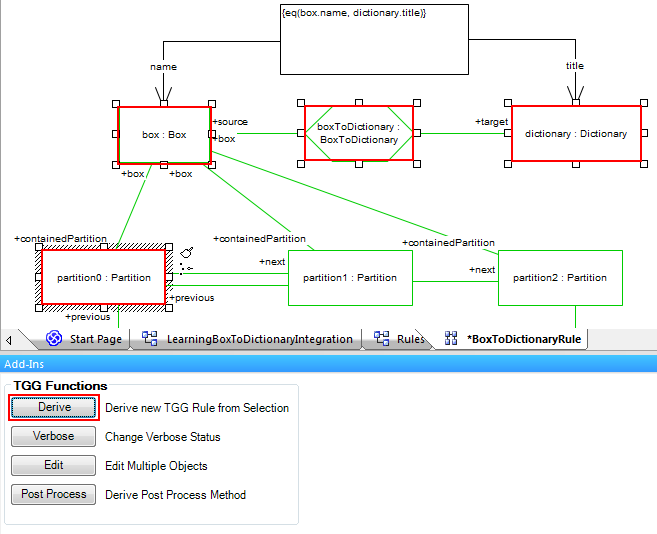
\includegraphics[width=\textwidth]{ea_selectPreDerivation}
  \caption{Derive from an existing TGG rule}
  \label{fig:derive_from_tgg_rule}
\end{center}
\end{figure}
\FloatBarrier

\item[$\blacktriangleright$] Add green instances of \texttt{Card} and \texttt{Entry} to the rule, and link them to their respective \texttt{partition0} and
\texttt{dictionary}. 

\item[$\blacktriangleright$] Quick-link from \texttt{card} to \texttt{entry} and create a new TGG Rule. You'll notice that the \texttt{correspondence type} menu
is empty -- we haven't defined one yet on the schema! Luckily, we're able to create one here. Select \texttt{create new correspondence type}, naming it
\texttt{CardToEntry} (Fig). 

Fig Here.

\item[$\blacktriangleright$] Your diagram skeleton should now resemble Fig.~\ref{fig:cardtoentry_1}. We're not done yet -- we still need to manipulate the
attributes of each element!

\vspace{0.5cm}

  \begin{figure}[htbp]
  \begin{center}
    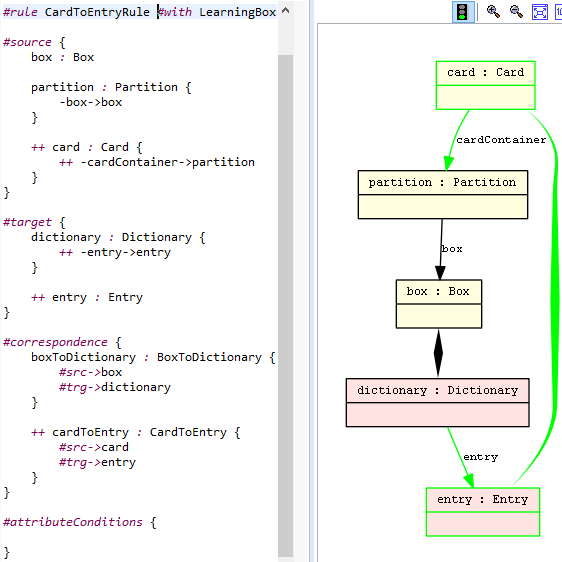
\includegraphics[width=\textwidth]{ea_cardToEntryRule}
    \caption{\texttt{CardToEntryRule} without attribute manipulation}
    \label{fig:cardtoentry_1}
  \end{center}
  \end{figure}

\end{enumerate}

We still need to create a series of constraints in order to specify how relevant attributes should be handled. Let's first define a construct for every
\texttt{entry.content}, \texttt{card.back}, and \texttt{card.face} EString values so that it's easy to (temporarily) persist the values during the
transformation. This will help us figure out how we should combine the front and back of each \texttt{card} as a single \texttt{content} attribute and,
in the opposite direction, help to separate the contents so that they may be split into \texttt{card.back} and \texttt{card.face}. Except
perhaps on a piece of paper so that you remember, you don't need to establish this syntax anywhere. 

Let's define \texttt{entry.content} as: \texttt{<word>:<meaning>}.  Syntax for \texttt{card.back} should therefore be \texttt{Question:<word>} and
similarly, \texttt{card.face} should be \texttt{Answer:<meaning>}. 


\begin{itemize}

\item[$\blacktriangleright$] We can now define three \emph{attribute constraints} to implement these. Luckily, we have two predefined constraints, \texttt{addPrefix} and
\texttt{concat} to help us. Use the toolbox again to create a new TGG Constraint, and add the following to your diagram:

  \item addPrefix(``Question '', word, card.face)
  \item addPrefix(``Answer'', answer, card.back)
  \item concat(``:'', word, meaning, entry.content)
  
\end{itemize}

Your rule should now resemble Fig.~\ref{fig:cardtoentry_2}, where ``Question'' and ``Answer'' are literals that will be translated directly to the relevant
elements, and \texttt{answer}, \texttt{word}, and \texttt{meaning} are temporary values to store information.

\vspace{0.5cm}

\begin{figure}[htbp]
\begin{center}
  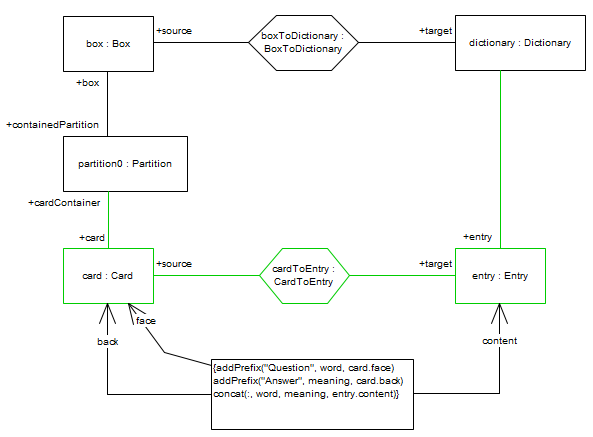
\includegraphics[width=\textwidth]{ea_completedCardToEntry}
  \caption{Attribute manipulation for \texttt{card} and \texttt{entry}}
  \label{fig:cardtoentry_2}
\end{center}
\end{figure}
\FloatBarrier


Our final task is to specify where a new \texttt{card} (when transformed from \texttt{entry} to \texttt{card}) will be placed.  We purposefully created three
partitions to match the three difficulty levels, but if you check the constraints drop-down menu, there is nothing that can implement this specific kind of
matching. We will therefore need to create our own constraint to handle this mapping.

\begin{enumerate}

\item[$\blacktriangleright$] Add one more constraint to your diagram but, instead of choosing a predefined constraint, click ``Add'' just below the
drop-down menu to create a custom one. Name it \texttt{IndexToLevel}, and enter the values given in Fig. \ref{fig:create_new_constraint}.

\vspace{0.5cm}

\begin{figure}[htbp]
\begin{center}
  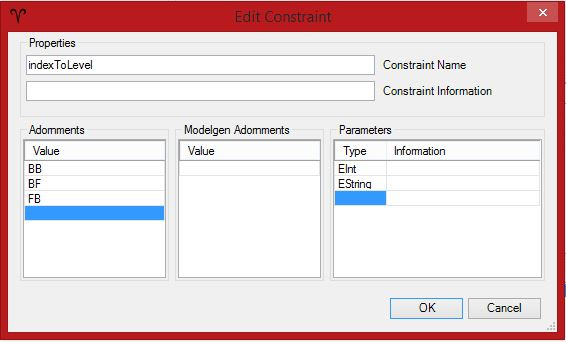
\includegraphics[width=\textwidth]{ea_uniqueConstraint}
  \caption{Create a user defined constraint \update}
  \label{fig:create_new_constraint}
\end{center}
\end{figure}
\FloatBarrier

\item[$\blacktriangleright$] Please note that this is just a specification of a custom constraint -- we still need to implement in Java! Since we're so close to
finishing this TGG Rule however, let's finish and export what we've made to Eclipse before doing so. Save the new constraint, then select it from the drop-down
menu in the TGG Constraint Dialog. Enter \texttt{partition0.index} as an \texttt{EInt} value, and \texttt{entry.level} as an \texttt{EString}.

\vspace{0.5cm}

\item[$\blacktriangleright$] Your completed TGG rule should resemble Fig.~\ref{fig:cardtoentry_complete}. Great work! You have now defined your link metamodel,
which nearly completes the TGG Triple required for a successful transformation. All that's left to do is implement the \texttt{IndexToLevel} constraint, and
give your transformation a test run.

\vspace{0.5cm}

\item[$\blacktriangleright$] Check out Fig.~\ref{fig:allReferences} in Section 4.3 to see how \texttt{BoxToDictionaryRule} is specified in the textual syntax,
or Fig.~\ref{fig:c2eDone} in Section 4.4 for the \texttt{CardToEntryRule}.

\end{enumerate}

\newpage

\vspace*{3cm}

\begin{figure}[htbp]
\begin{center}
  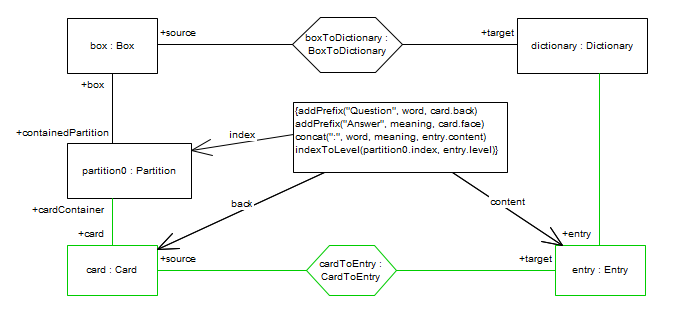
\includegraphics[width=\textwidth]{ea_cardToEntryComplete}
  \caption{\texttt{CardToEntryRule} with complete attribute manipulation}
  \label{fig:cardtoentry_complete}
\end{center}
\end{figure}


